\section*{Hypothesis}
Our hypothesis is that parallelising our code through coloring and running each color on the GPU simultaneously will provide a massive performance increase.


GPGPU `is the utilization of a graphics processing unit (GPU), which typically handles computation only for computer graphics, to perform computation in applications traditionally handled by the central processing unit (CPU)'\cite{gpgpu}.
GPU's are ideal for the smoothing algorithm that we have been provided with since although they can only process independent vertices and framgements they can process many of them in parallel and achieve SIMD performance. The transistors of a GPU are devoted to data processing(mainly integer and floating point)\cite{lec7}.

% TODO: WRITE A BIT FROM http://docs.nvidia.com/cuda/cuda-c-programming-guide/index.html - hardware impl section

Since we can colour our mesh and run verticies of the same colour on in parallel the GPU seems like a natural choice for optimisation. Furthemore the smoothing algorithm makes use of many floating point operations and so we should see a very large speed up from just porting to the CPU alone.

The CUDA Toolkit provides a comprehensive development environment and allows for easy migration of code.

\subsection*{Colouring}
We cannot independently smooth all verticies in the mesh simultaniously since a vertex depends on it's adjacent verticies. If these were smoothed at the same time the results would not be correct and so these must be locked down. We can however colour verticies of the mesh and run each independent set simultenously on the GPU.
Coloring is the first step that must be performed when porting the code across to the GPU.
We will experiment with a greedy algorithm that finds the first possible colour a vertex can fall in, and thus may not prove to be an optimal solution but will provide satisfactory results.


\subsection*{Migration to GPU}
In order to run the code on the GPU we must serialise 2D data structures. For example consider a vector of vectors:
\begin{verbatim}
  std::vector< std::vector<size_t> > colours = {[1, 5, 9, 2],
                                                [0, 4, 8],
                                                [3, 6, 7]};
\end{verbatim}
Since we do not have access to the standard library on a GPU the easiest and most efficient option is to turn this into a 1D array.
\begin{verbatim}
  size_t[] colours = {1, 5, 9, 2,
                      0, 4, 8,
                      3, 6, 7};
  size_t[] colour_indicies = {0 , 4, 7, 10};
\end{verbatim}
In each case must add an extra indices array, in this case \verb!colour_indicies!, to exactly where the beginning of each colour is in \verb!colours!. The array must be of size one larger than the number of items so that we can perform size
calculations of the individual groups inside for looping purposes.

Next we must copy input data from the CPU memory to GPU memory which can be done with the \verb!cuMemAlloc! function to allocate memory, \verb!cuMemcpyHtoD! to copy from host to device and a similar method to copy data back. All setup code for running on the GPU is in \verb!CUDATools.h!

Finally we must adapt the smoothing algorithm for the GPU in a number of steps:
\begin{itemize}
  \item \textbf{Modify the code to smooth a single vertex rather than looping through them all.} \\
        We can calculate the vertex id easily using block and thread indexing like so:
        % Don't adjust the indenting on this, verbatim is irritating!
        \begin{verbatim}
    const size_t threadID = blockIdx.x * blockDim.x + threadIdx.x;
    if(threadID >= NNodesInSet)
      return;
    size_t vid = colourSet[threadID];
        \end{verbatim}
        We must be careful to ensure that we do not access beyond the end of arrays and so the if statement above checks this for us.
  \item \textbf{Modify mesh methods for running on the GPU}. \\
        Since we will not have access to the mesh object on the GPU we will no longer be able to call methods such as \verb!mesh->isCornerNode(vid);!. All methods needed by the smoothing algorithm must be declared as \verb!__device__! methods and re-written.
  \item \textbf{Use constant memory}
        We will store our device data in constant memory on the GPU. The reason behind this is that Nvidia hardware can broadcast a single memory read to each half warp so if threads in a half warp request data from the same address then the GPU will only generate one load request.\cite{const_mem} It does this by splitting each half warp into as many separate requests as there are different memory addresses in the initial request, decreasing throughput by a factor equal to the number of separate requests.\cite{half_warp_broadcast} This will save a lot of traffic compared to global memory.
        Furthermore constant data is cached on the GPU so if the other half warp also needs the data it can get it from the cache rather than the memory.

\end{itemize}



It is however, not enough to stop at just running the code on our GPU. We must also then optimise for the GPU to achieve maximum performance. Therefore we propose the following.

\subsection*{Branching}
Unlike CPU cores GPU's offer no branch prediction or speculative execution.
When a multiprocessor is given one or more thread blocks to execute, it partitions them into warps (32 parallel threads), and these execute one common instruction at a time.
At branch statements threads can diverge however, the warp will serially execute each branch path taken for all threads (but just disabling them) and when paths complete the threads will converge.\cite{cuda_guide}. This will kill the performance of the GPU if many threads within a warp.

A major source of branching in the smoothing algorithm comes from the fact that different vertices have different numbers of neighbours. The three main loops (calculating worst coords, calculating the new worst coords, and assembling matrices A \& q) all depend upon looping over a vertices neighbours and thus each warp will end up executing the loop the maximum number of neighbours times.

We will therefore investigate the following:
\begin{itemize}
  \item \textbf{Minimising branching}
                In order to avoid this we will investigate minimising the branches by ordering the individual vertices in order of the number of neighbours they have. This will reduce branching since in most warps all threads will process vertices with the same degree and only a few unlucky warps that have a transition in number of neighbours will do some unnecessary work.
                For example if the vertices in colour 0 were 1, 4, 6, 7, 10, 12 and we have 0, 4, 6, 12 have 6 neighbours, 1 and 7 have 5, and 10 has 4 we would re-order them to be 10, 1, 7 0, 4, 6, 12.

  \item \textbf{Removing corner nodes during colouring}
                The smoothing algorithm bypasses any corner nodes and so we can avoid the conditional branch:
                % Don't adjust the indenting on this, verbatim is irritating!
                \begin{verbatim}
  if(isCornerNode(vid)) {
    return;
  }
                \end{verbatim}
                By factoring out corner nodes during the colouring phase it removes the need for this branch entirely and so should hopefully provide a slight speed up.
\end{itemize}

\subsection*{Pinning}
Host data allocations are pageable by default which means that the GPU cannot access data directly from pageable host memory. When a data transfer from pageable host memory to device memory is invoked, the CUDA driver must first allocate a pinned host array, copy the host data to the pinned array, and then transfer the data from the pinned array to device memory\cite{transfer}, as illustrated in Figure ~\ref{fig:pinning}.
\begin{figure}[H]
  \centering
  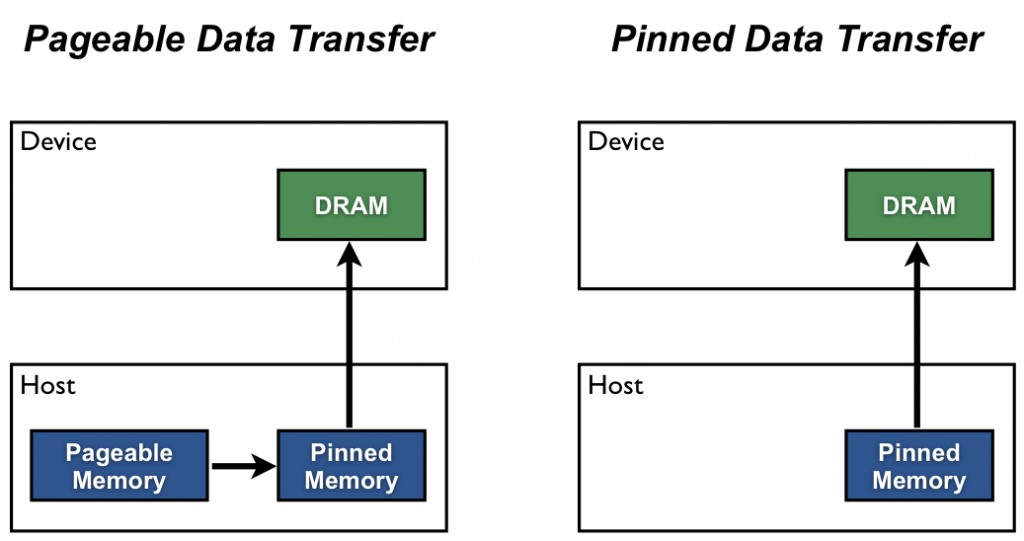
\includegraphics[scale=0.3]{images/pinning}
  \caption[pinning]{GPU Data Transfers\cite{transfer}}
  \label{fig:pinning}
\end{figure}
Pinned memory is used as a straging area for transfers and we can avoid this cost by directly allocating our host arrays (e.g colours) in pinned memory.

Since we do not know the size of our 2D data arrays we will allocate all our data in normal memory using the standard library data structurs and then in a pre-processing stage call a \verb!pin_data! method on the mesh and similarly with the colours.
With extra code our data structures could be pinned straight away, however we perform this pre-processing stage as a comprimise to allow us to spend our time on GPU optimisations rather than speeding up the CPU code which does not count in the benchmark timings.

We can easily lift the code we will write for serializing data structures \verb!CUDATools.h! into the Mesh, so this should hopefully reduce time spent on this optimisation.
\subsection{Threads Per Block}
Every thread block is mapped to one or more warps, which contains 32 parallel threads that are launched together. When launching a kernel in CUDA we can specify the number of blocks, and threads per block. Of course the total number of threads must be greater than or equal to the number of vertices in each colouring (so as to process all vertices), but we can vary the ratio of blocks and threads to find a sweet spot.

The number of threads should be a multiple of the warp size, which is 32 for the GeForce GT 330, as it will ensure that the GPU is not wasting computation on under-populated warps. The GPU will switch between warps to hide memory latency\cite{threads_atomics}, and so if the number of threads per block is too small there may not be a warp to schedule while another warp is waiting for a memory access. However, too large a number of threads per block will result in there not being enough blocks to use every streaming multiprocessor available thus under-utilising the hardware available.